\section{Introduction}
% statement of problem
% purpose and significance

Self-assembly is a powerful tool for creating complex materials with tailored particle interactions.
Systems order with interactions as simple as hard-particle excluded volume \cite{Damasceno_2012_Science} and as complex as DNA-programmed origami \cite{Winfree_1998_Nature}. 
While much research has been focused on understanding how to design highly-specific building blocks and predict assembled structure, relatively little work has been focused on optimizing specificity in self-assembly system design.

Put another way-- 
\textbf{what is the minimal set of instructions needed to achieve targeted, self-assembled complexity?}

%To investigate this question, we use a system of folding nets (of the five Platonic solids) with non-specific edge interactions.
%Previous molecular dynamics studies of this system have shown that compact nets with more leaves are more likely to be able to fold into (i.e. assemble) the Platonic solid from which they were derived (i.e. their target structure).   
%Authors observe that in these nets, folding pathways are enabled by the formation of local, native bonds, mirroring phenomena observed in protein folding.
%
%This suggests that though the interactions are not specific, the combination of geometry and attraction serve to make some of these bonds more effective than others.
%In turn, this suggests that it is possible to identify bonds that are more critical to assembly than others. 
%If we are able to rank the importance of interactions on the yield of an assembly pathway, then it stands to reason that we can determine which interactions are the minimally sufficient set needed to guide assembly into a target structure. 

%Self-assembly is a powerful tool for creating materials by design.
%Systems of simple particles with programmed interactions are capable of creating a rich complexity of structures and behaviors.
%One of the key challenges of modern materials design is understanding self-assembly to use it to create even more complex structures.
%
%Here, we propose using a simple folding model of nets to develop methodology for identifying ``high information bonds''-- i.e., bonds that are critical to avoid kinetic traps and enabling further assembly.
%We propose using the methods and information metrics developed to then develop an ``information efficiency'', to determine the minimal amount of programmed interactions required to still reliably reach a target state.


%Colloidal-scale self-assembly is of particular interest. 
%Larger than atoms, colloids experience thermal fluctuations (and thus are well-characterized by statistical thermodynamics).
%Additionally, much research has been spent characterizing their behavior.
%They are easily synthesized in experiments, and can be simulated simply.

%Recent innovations in DNA-programmed assembly have demonstrated the ability to assemble specifically ordered arrangements of particles with both high complexity and high accuracy.
%The sequence-specific binding property of DNA can be applied to direct the assembly behavior of colloidal particles at the nanoscale.
%Theoretical work has shown that this powerful assembly shouldn't be limited to DNA systems, but rather accessible to any system with sufficiently specific interactions (including colloids) \cite{Reinhardt_2014_PRL}. 
%
%However, such highly-programmed assembly is prone to two problems.
%\begin{enumerate}
%\item Performance of assembly is highly reliant upon kinetics to avoid mis-matches or multiple nucleation events
%\item Exacting level of specificity required is currently only achievable with DNA methods
%\end{enumerate}

% could include something here about the relative citations on different papers-- there's something missing here; everything is too specific?

%Such an approach would provide a powerful toolkit for scientists looking to engineer colloidal systems with addressable complexity.

%\textbf{Key question: How can we \textit{most efficiently} direct a system to self-assemble?}


\section{Background}

% =====
% SELF-ASSEMBLY, GENERALLY
% =====

Self-assembly is the process by which individual components arrange themselves into an ordered structure via free energy minimization \cite{Whitesides_2002_Science}.
This ordered structure is determined by the inter-particle interactions and assembly environment, and much recent work has focused on tuning these parameters to achieve target structures \cite{Boles_2016_ChemRev}. 
With advances in material synthesis techniques, complex building blocks can now be made with nano- and micro-precision.
Correspondingly, there has been a focus in the literature to understand the role of building block properties on the bulk structure assembled.

At the colloidal scale, seemingly simple additions of anisotropic interactions to building blocks can yield complex structures \cite{GlotzerSolomon_2007_Nature}.
Hard particles with shape can assemble a rich variety of structures \cite{Damasceno_2012_Science}, even in the absence of explicit interactions between particles other than excluded volume.
Later work described this as the effect of an effective entropic patchiness caused by shape interactions \cite{vanAnders_2014_ACSNano}.

Even when specific interactions are added, they do not need to be complex for small changes to lead to very different structures.
Adding explicit attractive patches to otherwise isotropic particles led to the formation of shapes, clusters, and rings, depending on the orientation of the patches \cite{Zhang_2004_NanoLetters}.
Later, Millan \textit{et al.} were able to access Archimedean tilings of regular polygons by incrementally adding attraction to guide assembly to target structures \cite{Millan_2014_ACSNano}.
However, even non-specific directional attractive patches can cause particles (in one case, nanoplates forming a superlattice) to self-assemble structures differing from those accessible via entropic forces alone \cite{Ye_2013_NatChem}.
Experimentally, DNA-mediated particle interactions are now a powerful tool for tailoring crystal structure of a uniform building block \cite{Park_2008_Nature}.

The diversity of structures that can be accessed from simple interactions is impressive, and there is still much to be understood about how inter-particle interactions impact the structure assembled.

\begin{figure}[t]
\begin{center}
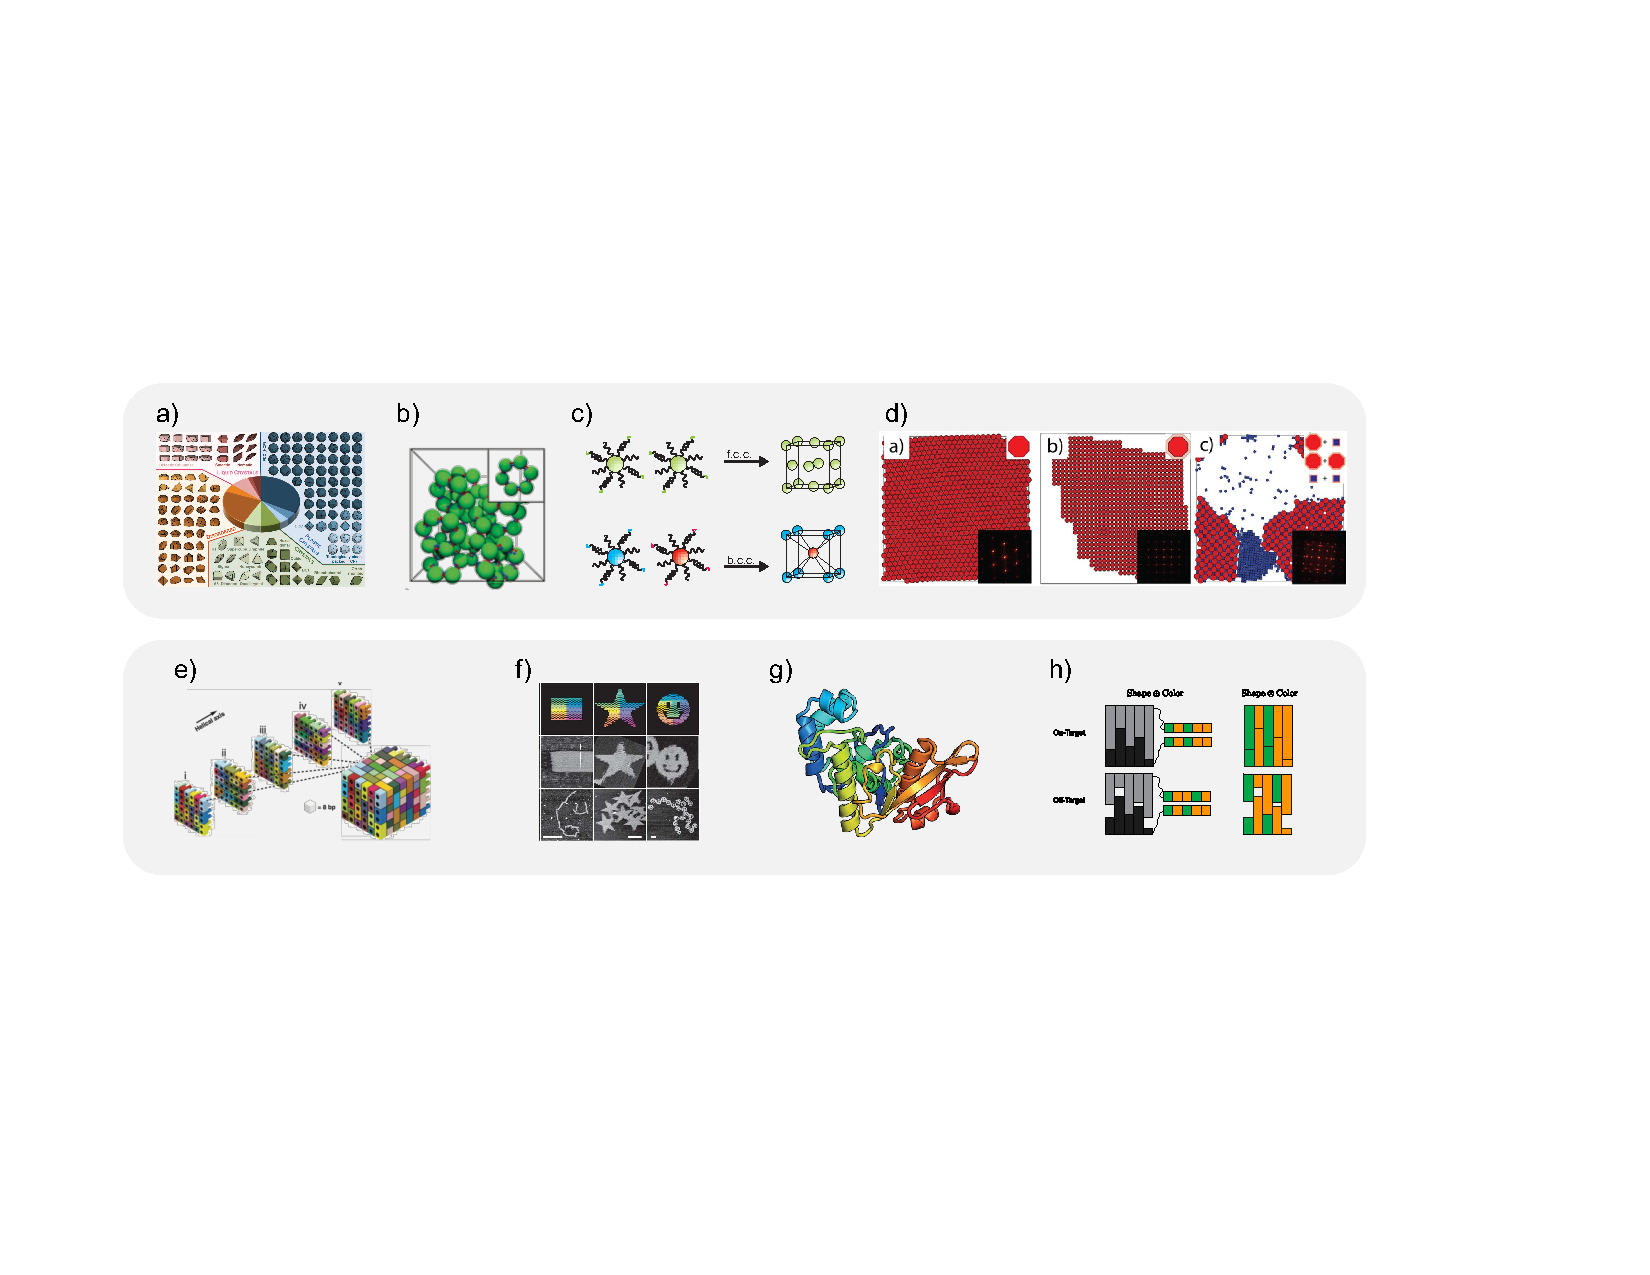
\includegraphics[width=6.5in]{../figures/1-LiteratureReview.pdf}
\caption{
\textbf{Self-assembly in the literature}:
Top: Simple interactions between particles can lead to a rich variety of assembled structures.
Systems shown: 
(a) ordered structures from hard polyhedra \cite{Damasceno_2012_Science};
(b) isotropic particles with attractive patches \cite{Zhang_2004_NanoLetters};
(c) crystal structure tailored with DNA-mediated assembly \cite{Park_2008_Nature};
(d) Archimedean tilings assembled from polygons with increasing bond specificity \cite{Millan_2014_ACSNano}.
Bottom: Programmable interactions can enable addressable complexity.
(e) DNA bricks assembled in a one-pot system with single-stranded DNA \cite{Ke_2012_Science};
(f) DNA origami \cite{Rothemund_2006_Nature};
(g) de novo protein design \cite{Huang_2016_Nature};
(h) theoretical calculation of chemical and shape bond instruction capacity \cite{Huntley_2016_PNAS}.
}
\label{fig:litreview}
\end{center}
\end{figure}

However, recent advances in synthesis of programmable DNA building blocks have now enabled significantly more complex interactions, resulting in self-assembly processes of addressable complexity.
In addressable systems, each particle has a specific location (address) that it is ``programmed'' to assemble into.
%Such assembly is as much a function of the kinetics of the process (e.g. annealing) as it is the thermodynamics of the interparticle interactions.

Biologically, we are familiar with specifically-programmed assembly in DNA replication or protein folding \cite{Dill_1993_CurrOpinStructBiol}.
Synthetically, though, the most well-known examples of addressable complexity are DNA-based.
``One-pot'' addressable self-assembly of DNA bricks uses the hybridization of complementary DNA sequences to construct addressable structures from a single pool of monomers \cite{Ke_2012_Science}.
Simulation results have shown that such one-pot self-assembly can succeed with highly simplified model subunits that lack the molecular details of DNA tiles, suggesting that similar design strategies should be possible in non-DNA-based synthetic systems \cite{Reinhardt_2014_PRL}.

In addition to using programmed DNA interactions between particles, programmed self-assembly can also refer to design of DNA strands or protein primary structures themselves.
DNA origami is perhaps the most well-known example of this \cite{Rothemund_2006_Nature,Winfree_1998_Nature}.
Given a target structure (such as the much-cited example of a smily-face), a DNA strand can be programmed that will fold precisely into the designed target \cite{Rothemund_2006_Nature}.
While some examples of protein design exist (e.g. \cite{Huang_2016_Nature}), it is possible that the additional challenge of designing structure from a set of 22 amino acid residues versus 4 nucleotide bases in DNA has limited its appeal as a designer system.

While much work has focused on designing interactions to tailor self-assembly, we must also note that simply having sufficiently-specific interactions does not guarantee a system will reach a target state.
If assembly temperature is too high, bonds may be unable to stably form; if the assembly temperature is too low, the system may be unable to sufficiently sample configuration space to reach the target structure.
Though the target maybe be the global free energy minimum, that does not mean that it can be reached kinetically.  
Temperatures and binding energies must be carefully tuned to enable systems to sufficiently sample possible configurations and escape kinetic traps while still enabling stability in the ground state (i.e. bonds do not spontaneously break).
In a noteworthy example, the yield of the one-pot DNA self-assembly system studied in \cite{Ke_2012_Science} was found via simulation to be highly sensitive to both temperature \cite{Reinhardt_2014_PRL} and the annealing protocol used \cite{Jacobs_2015_PNAS}. 

A collection of the self-assembly results discussed here and in the remainder of this proposal is shown in Figure \ref{fig:litreview}.
